\section{Historical evaluation}
\label{sec:research}

Fixed configurations run continuously over 2015-2023. Ranking uses the
72 monthly returns from 2018-2023; six annual slices assess variation without
resetting capital or reselecting parameters. Longer estimators can delay
activation beyond the nominal 2014 warm-up.

\begin{figure}[H]
  \centering
  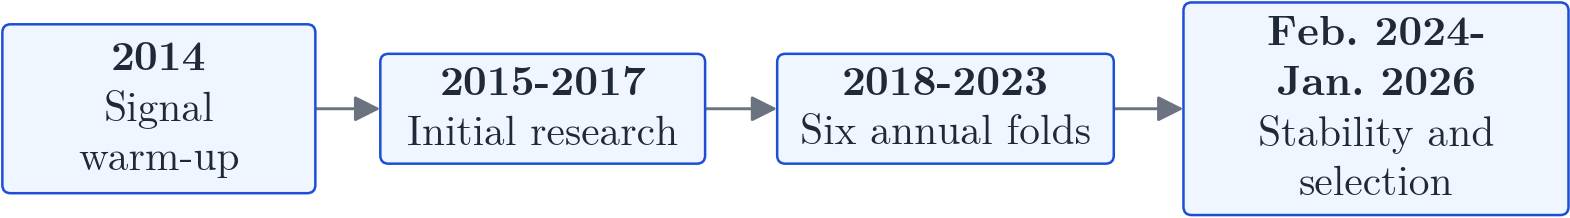
\includegraphics[width=\reportfigurewidth]{figures/historical_evaluation_timeline.png}
  \caption[Historical evaluation timeline]{Historical windows. The test portfolio starts on January 31, 2024
  and produces 24 monthly returns.}
  \label{fig:evaluation-timeline}
\end{figure}

We ranked 5,760 momentum configurations by net return, varying formation,
position counts, sizing, exposure, buffers, turnover thresholds and sector
neutrality. Candidate \#1292 ranked fourth, then led the top-five shortlist
in the test window (\cref{tab:momentum-shortlist}).

\begin{table}[htbp]
  \centering
  \begin{threeparttable}
  \small
  \setlength{\tabcolsep}{5pt}
  \begin{tabular}{lrrrrr}
    \toprule
    Candidate & Validation & Validation & Test return & Test & Test \\
              & return rank & return & & Sharpe & drawdown \\
    \midrule
    \#1436 & 1 & $+78.02\%$ & $+108.11\%$ & 1.25 & $-16.87\%$ \\
    \#1712 & 2 & $+74.47\%$ & $+95.34\%$  & 1.17 & $-16.23\%$ \\
    \#1724 & 3 & $+74.44\%$ & $+103.37\%$ & 1.24 & $-15.40\%$ \\
    \textbf{\#1292} & \textbf{4} & $\mathbf{+73.79\%}$ &
      $\mathbf{+140.37\%}$ & \textbf{1.28} & $\mathbf{-16.07\%}$ \\
    \#1424 & 5 & $+70.72\%$ & $+101.52\%$ & 1.20 & $-16.69\%$ \\
    \bottomrule
  \end{tabular}
  \caption[Momentum shortlist: validation and test results]{The return-focused momentum shortlist. Validation covers
  January 2018-December 2023; the test window covers
  February 2024-January 2026. Returns are cumulative and net of modeled costs.}
  \label{tab:momentum-shortlist}
  \end{threeparttable}
\end{table}

In the test window, \#1292's volatility was 38.27\%, versus 10.63\% for the
benchmark. January 2026 supplied 48.37\% of cumulative profit; the preceding
23 months still returned 72.48\%, versus 44.94\%. Annualized compound return
was 55.04\%, against
21.26\%; beta was 1.49, Treynor 0.329 and Information Ratio 0.881.
Annualized CAPM alpha was 22.17\% ($p=0.439$), not statistically significant
at the 5\% level.

\begin{figure}[H]
  \centering
  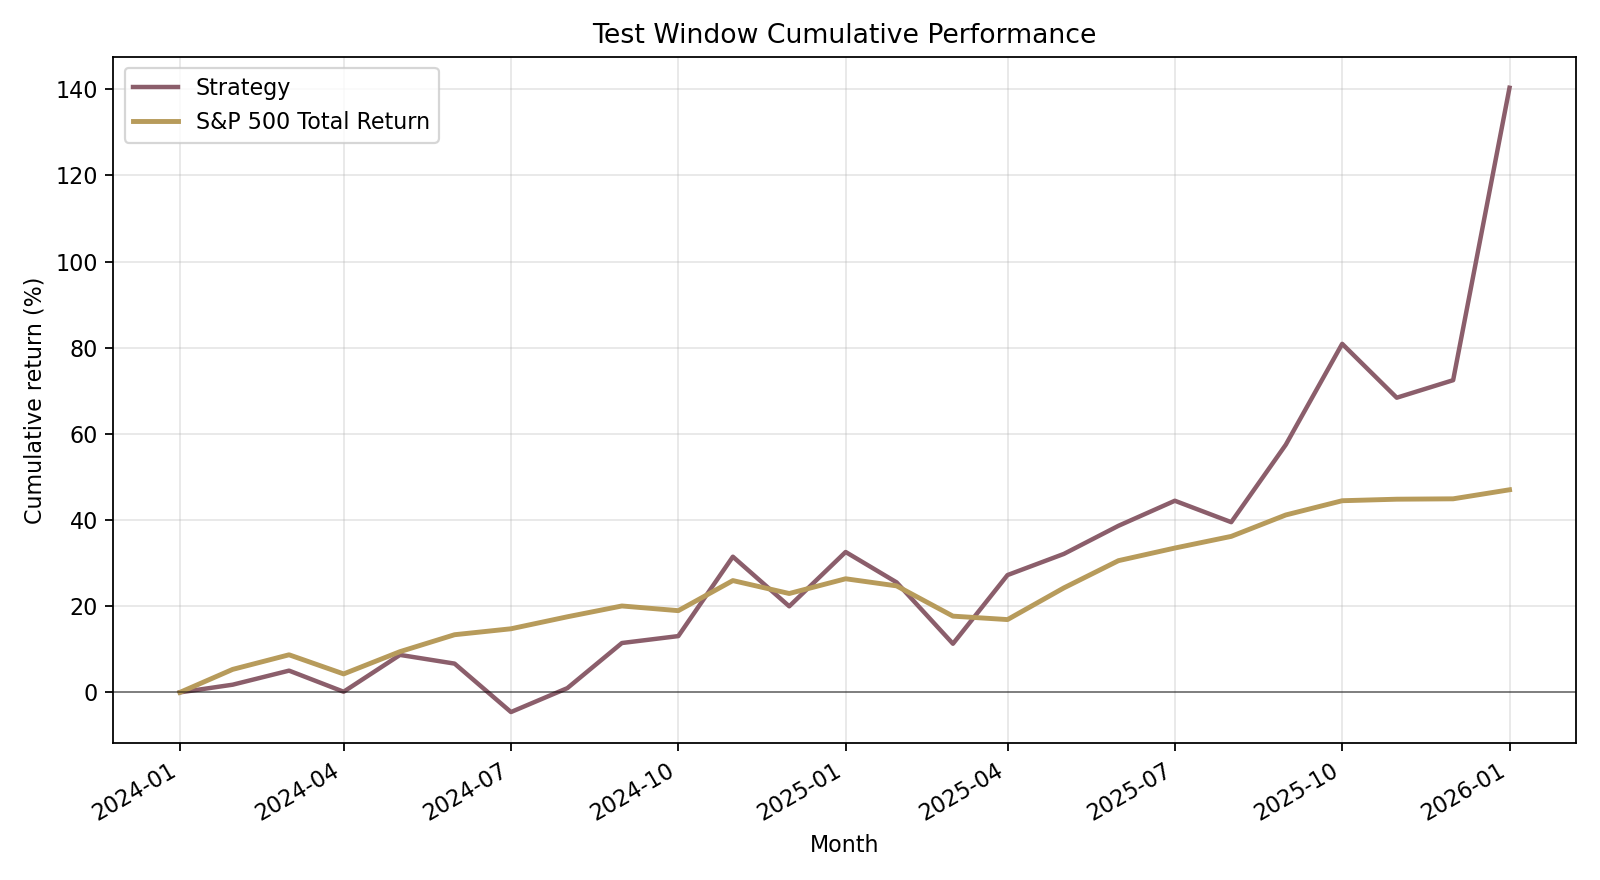
\includegraphics[width=\reportfigurewidth]{../outputs/backtest/strategies/momentum/figures/test_window/cumulative_performance.png}
  \caption[Momentum \#1292: cumulative net performance, Feb.~2024-Jan.~2026]{Momentum \#1292: cumulative net performance, Feb.~2024-Jan.~2026.}
  \label{fig:historical-performance}
\end{figure}

\begin{figure}[H]
  \centering
  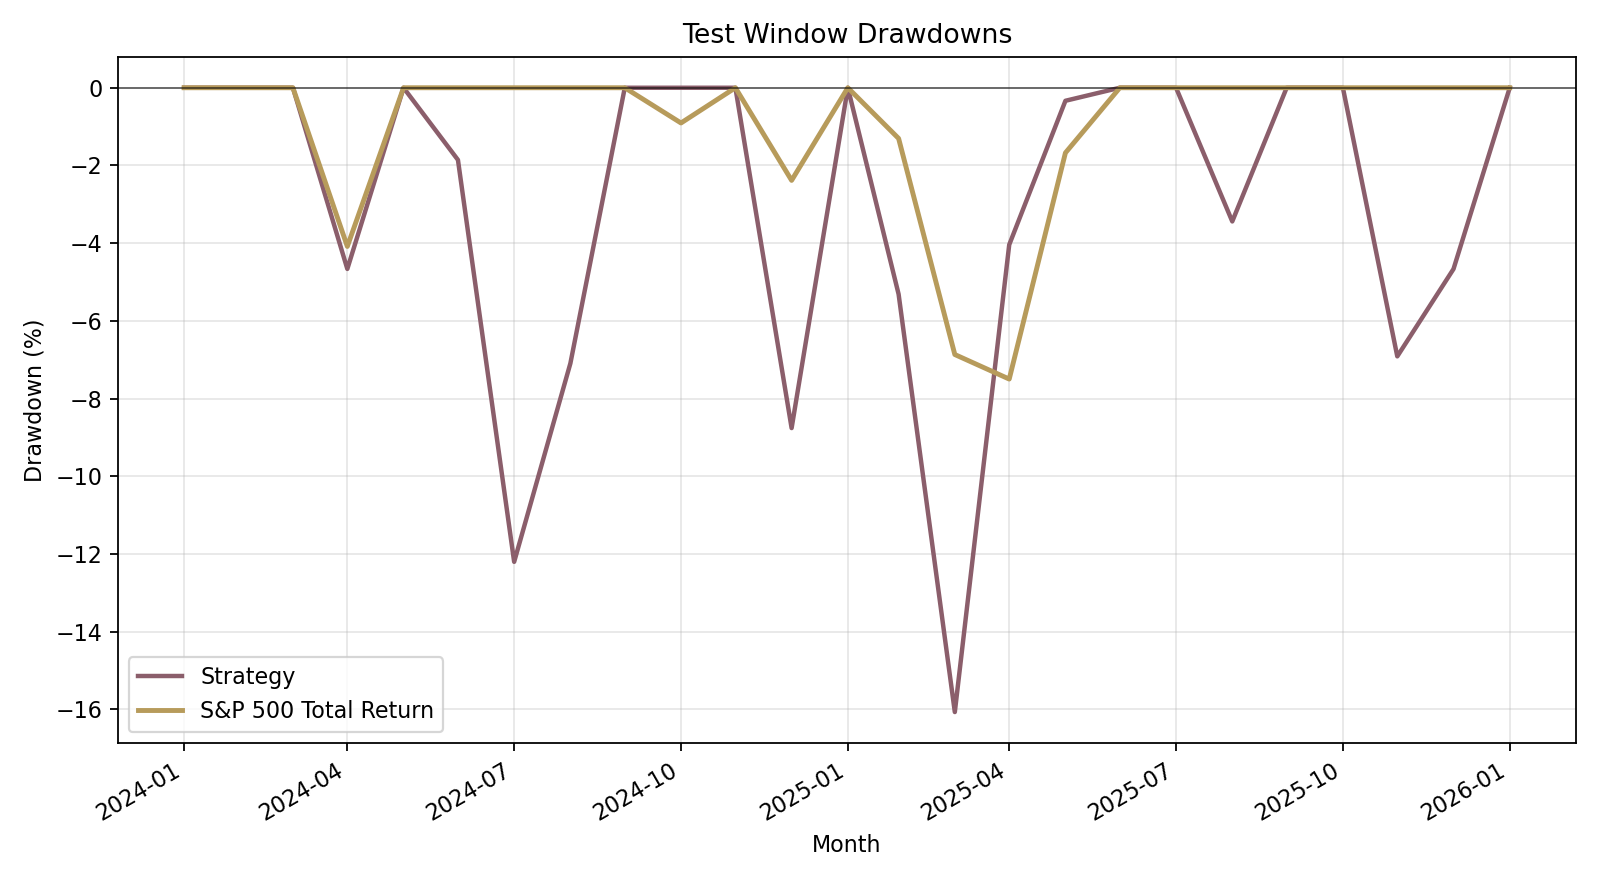
\includegraphics[width=\reportfigurewidth]{../outputs/backtest/strategies/momentum/figures/test_window/drawdown.png}
  \caption[Momentum \#1292: month-end drawdown, Feb.~2024-Jan.~2026]{Momentum \#1292: month-end drawdown, Feb.~2024-Jan.~2026.}
  \label{fig:historical-drawdown}
\end{figure}

\subsection{Costs and alternatives}

The test run placed 371 orders, costing \$742 in fees, \$6,837 in spreads and
\$17,693 in loan interest. Return before fees and spreads, but after financing,
was 142.57\%, versus 140.37\% net. Monthly turnover averaged 1.165 times
pre-trade equity, counting absolute purchases and sales at reference prices.
Low/base/high spread cases returned 140.68\%/140.37\%/140.06\%; these vary
only the modeled spread coefficient.

We compared three other families on the same validation dates and accounting
basis (\cref{tab:alternative-validation}); drawdown uses the initial wealth
level and monthly marks.

\begin{table}[htbp]
  \centering
  \begin{threeparttable}
  \small
  \setlength{\tabcolsep}{5pt}
  \begin{tabular}{lrrrrr}
    \toprule
    Strategy & Ranked candidates & Candidate & Net return & Sharpe & Drawdown \\
    \midrule
    Momentum & 5,760 & \#1292 & $+73.79\%$ & 0.420 & $-26.36\%$ \\
    Reversal & 1,152 & \#1123 & $+50.79\%$ & 0.327 & $-31.50\%$ \\
    Low volatility & 1,152 & \#598 & $+15.49\%$ & 0.094 & $-22.75\%$ \\
    Sector momentum & 967 & \#881 & $+69.34\%$ & 0.556 & $-16.42\%$ \\
    \bottomrule
  \end{tabular}
  \caption[Selected validation results by strategy family]{Selected validation results for January 2018-December 2023.
  The alternative rows show each family's cumulative-return leader; momentum
  shows our selected configuration. Sector momentum attempted 1,296 compatible
  configurations, of which 329 were execution-infeasible.}
  \label{tab:alternative-validation}
  \end{threeparttable}
\end{table}

\FloatBarrier
\textbf{Reversal} buys prior-month losers and shorts winners. Return and
Sharpe leader \#1123 turned over 132.85 times equity and paid \$66,879 in
fees and spreads; median grid return was $-6.30\%$.

\textbf{Low volatility} buys the least volatile stocks and shorts the most
volatile, using 60 months with at least 24 observations. Only 39 of 1,152
configurations profited; median return was $-36.94\%$. Sharpe leader \#599
scored 0.095 and lost money in every year from 2019 through 2023.

\textbf{Sector momentum} ranks equal-weight sector returns and trades whole
baskets; the leaders use three long and three short sectors. Sharpe leader
\#763 returned 45.81\%, with Sharpe 0.598 and drawdown 7.23\%. Our return-first
comparison favored momentum. Infeasible configurations failed position counts
under scaled whole-share execution and receive no investment returns.

\begin{samepage}
\textbf{Monthly trend} ranks price relative to its monthly moving average.
Its strategy and grid are implemented, but the grid search was not run;
we draw no empirical performance conclusion.

\end{samepage}

Shared samples and related parameters create selection bias; annual slices
are not independent economic regimes. Their returns appear in
\cref{tab:annual-folds}.

\begin{table}[H]
\centering
\begin{threeparttable}
\small
\begin{tabular}{@{}lrrrr@{}}
\toprule
Year & Momentum \#1292 & Reversal \#1123 & Low volatility \#598 & Sector momentum \#881\\
\midrule
2018 & $-18.89\%$ & $+1.69\%$ & $+21.15\%$ & $-9.60\%$\\
2019 & $+3.09\%$ & $+28.91\%$ & $-1.65\%$ & $+9.13\%$\\
2020 & $+30.07\%$ & $+14.73\%$ & $-0.53\%$ & $+22.94\%$\\
2021 & $+14.49\%$ & $+12.95\%$ & $-1.31\%$ & $+14.29\%$\\
2022 & $+1.62\%$ & $-12.76\%$ & $+0.33\%$ & $+18.01\%$\\
2023 & $+37.35\%$ & $+1.75\%$ & $-1.59\%$ & $+3.52\%$\\
\bottomrule
\end{tabular}
\caption[Annual validation returns, 2018-2023]{Annual net returns within the continuous 2018-2023 validation run.}
\label{tab:annual-folds}
\end{threeparttable}
\end{table}
\FloatBarrier
